\documentclass[a4paper, 12pt]{article}
\usepackage{fullpage}
\usepackage[utf8]{inputenc}
\usepackage[english]{babel}
\usepackage{latexsym}
\usepackage{color}
\usepackage{amssymb}
\usepackage{amsmath}
\usepackage{graphicx}
\usepackage{fancyhdr}
\usepackage{caption}
\usepackage{subfigure}


\pagestyle{fancy}
\fancyhf{}
\fancyhead[RE,LO]{Project 2: Learning of Grid Cells}
\headsep=15mm

\title{Project 2: Learning of Grid Cells}
\author{Claus Lang, Can Eren Sezener, Claudia Winklmayr}
\date{09.02.2016}


\begin{document}
\maketitle

\paragraph{Abstract:}
Grid cells, located in rats medial entorhinal cortex (mEC), show increased firing activity when the animal enters specific regions of the environment. The resulting firing maps show a characteristic hexagonal grid pattern. In our project we implement a computational model for the development of grid cells, introduced by Kropff and Treves. We simulate a rat exploring a square environment at constant speed. The $x$ and $y$ coordinates of its loactions serve as input for a layer of 400 place units. The output layer then recieves a weighted sum of the place cells activity to compute the activation of 100 grid cells.
 

\section{Introduction}
There are various types of neurons that serve to encode an animals spacial location. Place cells - located in hippocampus - were discovered in the 1970s by O'Keefe and Dostrovsky. Place cells show increased activity when the animal enters a specific region of the environment - the so called place field.\newline
Grid cells - located in medial entorhinal cortex (mEC) were then discovered in 2005. In contrast to place cells they are activated at various locations and their firing maps show a characteristic hexagonal grid pattern. Different grid cells can be distinguished by their spacing, orientation and spacial phases. Neighboring grid cells usually show similar and orientation. \newline
It is assumed that grid cells perform a path integration task, taking into account the rats position, speed and direction. Visual information on the other hand plays at most a secondary role in the formation of the grid pattern. \newline
The Kropff and Treves model assumes places cells as the basis for grid cell development. The place cells take as input the $x$ and $y$ coordinates of a virtual rat exploring a square environment of 125cm length. Every output unit then receives input from all place cells and the weights connecting input and output neurons are updated by a Hebbian learning rule. 
%
%
%
\section{Model}
The model consists of a layer of 400 input neurons (simulating place cells) and 100 ouput neurons (simulation grid cells), every unit of the input layer being connected to every unit of the output layer. By $w_{ij}$ we denote the weight of the connection between the $j$-th input unit and the $i$-th output unit. 
\begin{figure}
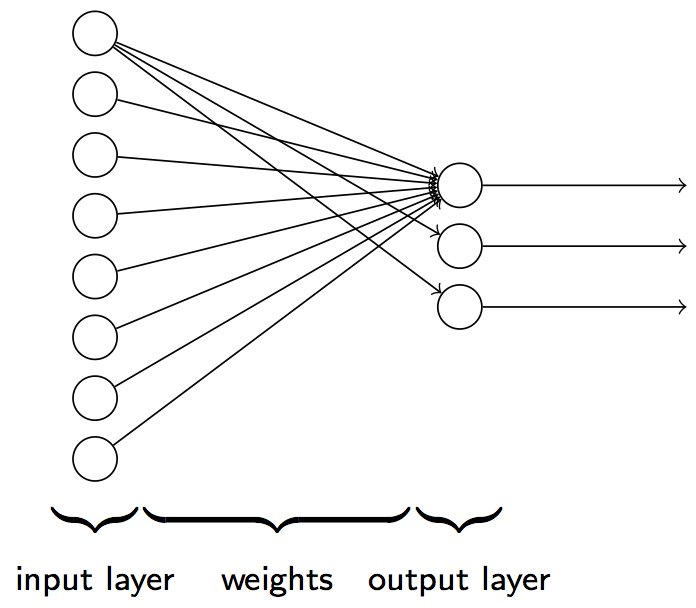
\includegraphics[width=0.5\textwidth]{model_overview.png}
\end{figure}
\subsection{Spacial Information}
\begin{figure}[h]
\begin{minipage}{0.5\textwidth}
	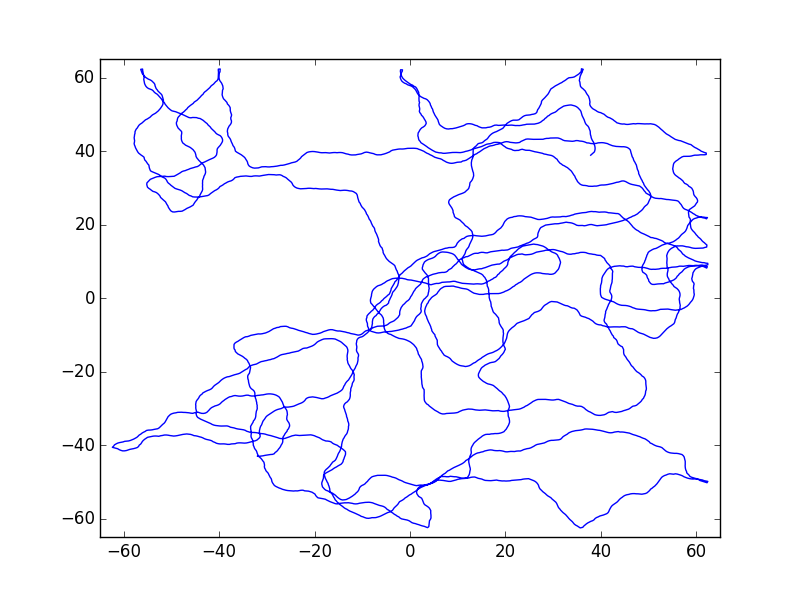
\includegraphics[width=5cm, height=5cm]{running_rat.png}
	\caption{\footnotesize{trajectory of the virtual rat exploring for 50 seconds}}
\end{minipage}
\begin{minipage}{0.5\textwidth}
To create the spacial coordinates that serve as input for the first layer of neurons, we simulate a rat exploring a square environment of size 125cm $\times$ 125cm at a speed of 0.4 m/s. At each timestep $\tau=$10ms we chose a new direction by randomly drawing an angle $\phi$ from a normal distribution, which is centered around the direction at the prvious timestep and has a standard deviation of 0.2rad.   
\end{minipage}
\end{figure}


\subsection{Input layer}
The input layer consists of 400 place units processing information about the rats location $\boldsymbol{x}(t)$ at a given time $t$. The firing $r_j^{in}(t)$ of each place unit is modeled by an exponential function centered around the cells prefered location $\boldsymbol{x}_j$. The respective fireing field's width is $\sigma_p=$ 5cm. 
	\begin{equation}
	r_j^{in}(t)=\exp\left(\frac{-|\boldsymbol{x}^t-\boldsymbol{x}_j|}{2\sigma_p^2}\right)
	\end{equation}
\begin{figure}[h]
\setlength{\abovecaptionskip}{5pt}
\setlength{\belowcaptionskip}{0pt}
\begin{minipage}[t]{0.3\textwidth}\vspace{0pt}
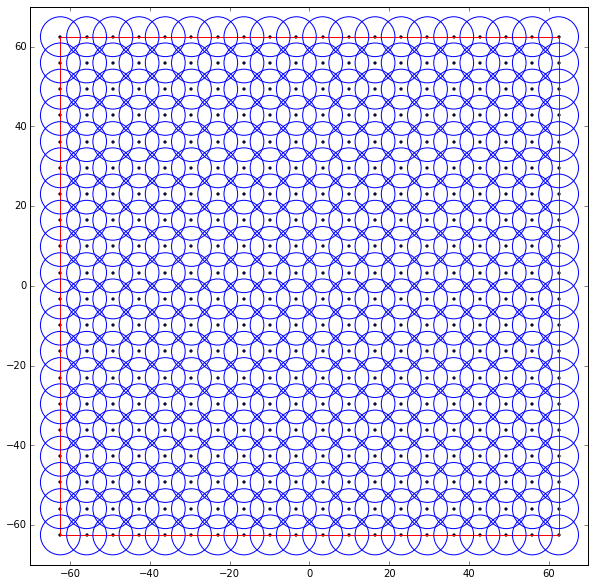
\includegraphics[width=4cm, height=4cm]{place_cell_locations}
\end{minipage}\hfill%
\begin{minipage}[t]{0.3\textwidth}\vspace{0pt}
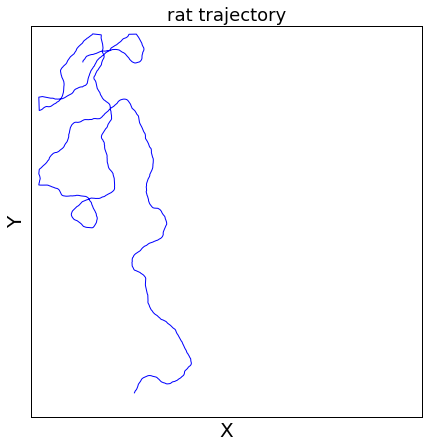
\includegraphics[width=4cm, height=4cm]{mouse_demo}
\end{minipage}\hfill
\begin{minipage}[t]{0.3\textwidth}\vspace{0pt}
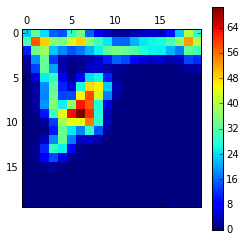
\includegraphics[width=5cm, height=5cm]{activity_demo}
\end{minipage}
\caption{\footnotesize{From left to right: (i) distribution of place fields across the environment, (ii) trajectory of the virtual rat and (iii) corresponding activity of place cells.}}
\end{figure}
%
%
%	
\subsection{Output layer}
At each timestep every output unit recieves as input a weighted sum $h$ of the activations of all place cells. For the $i$-th output unit this takes the form: 
	\begin{equation}
	h_i(t)=\sum_jw_{ij}r_j^{in}(t).
	\end{equation}
This input is then subject to an dynamic adaptaion process, during which we also determine parameters $g$ and $\mu$ which controll the mean firing activity across neuons as well as the sparsity. To calculate the final output $r_i^{out}(t)$, we then use a nonlinear activation function:
	\begin{equation}
	r_i^{out}(t) = f(r^+(h_i(t)); g,\mu).
	\end{equation}

\noindent The crucial point for the developement of grid cells is that we do not directly use the value $h_i(t)$ to calculate the output laver activity but first subject it to the following adaptation process: 
	\begin{eqnarray}
	\tau^+\frac{d}{dt}r^+ &=& h_i(t)-r^+(t)-r^-(t)\\
	\tau^-\frac{d}{dt}r^- &=& h_i(t)-r^-(t)
	\end{eqnarray}
The control parameters $g$ and $\mu$ are determined by itereation. $g$ serves to keep the mean activity across neurons - defined via $a= \frac{1}{400}\sum_ir_i^{out}$- within a 10\%-range from the value $a_0$. The parameter $\mu$ respectively controls the sparsity $s=\frac{(\sum_ir_i^{out})^2}{\frac{1}{400}\sum_i (r_i^{out})^2}$ and keeps it within a 10\% error bound of the value $s_0$. At each iteration step $g$ and $\mu$ are updated in the following way: 
	\begin{eqnarray}
	\mu^{t, l+1} &=& \mu^{t,l}+b_\mu(a^{l}-a_0)\\
	g^{t,l+1} &=& g^{t,l}+ b_gg^{t,l}(s^l-s_0)
	\end{eqnarray}
\noindent $l$ indicates the step of the iteration. The updating process is stopped if both $a$ and $s$ fall within the 10 \% error bound of $a_0$ and $s_0$. In any case the updating process stops after 100 iterations. 
	
\begin{figure}[h]
\setlength{\abovecaptionskip}{5pt}
\setlength{\belowcaptionskip}{0pt}	
	\begin{minipage}[t]{0.5\textwidth}\vspace{0pt}
	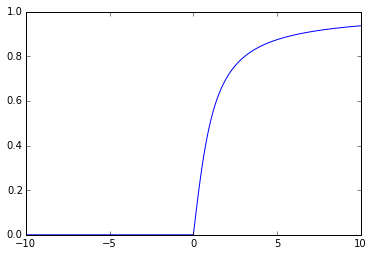
\includegraphics[width=5cm, height=4cm]{output_function.png}
	\caption{\footnotesize{Activation function for output neurons}}
	\end{minipage}
\hfill
	\begin{minipage}[t]{0.5\textwidth}\vspace{20pt}
	\begin{tabular}{c|cccccccc}
	& $a_0$ & $s_0$ & $\mu^{0,0}$ & $g^{0,0}$ & $b_\mu$ & $b_g$& $\tau^+$ & $\tau^-$\\
	\hline\\
	& 0.1 & 0.3 & 0 & 4.5 & 0.01 & 0.1& 0.1 & 0.3\\
	\end{tabular}
	\caption{\footnotesize{Default parameters for adaptation dynamics}}
	\end{minipage}
\end{figure}	

\noindent Using the above introduced expressions we can now write down the activation function in its complete form: 
	\begin{equation}
	r_i^{out}(t)=\frac{2}{\pi}\arctan(g(r_i^+(t)-\mu))\Theta( r_i^+(t)-\mu)
	\end{equation}
The factor $\frac{2}{\pi}$ serves to normalize the output to a value between 0 and 1 while the Heaviside step-function $\Theta$ makes sure that we only recieve positive output-values. 
%
%
%
\subsection{Weights}
The weights connecting input and output layer are initially being drawn from a uniform distribution in $[0,1]$ and normalized to unity i.e. for every output unit $i$ we impose $\sum_jw_{ij}=1$. At each timestep the weights are then updated using a Hebbian learning rule:  
\begin{equation}
w_{ij}(t+\Delta t)= w_{ij}(t)+ \epsilon(r_i^{out}(t)r_j^{in}(t)-\overline{r}_i^{out}(t)\overline{r}_j^{in}(t))
\end{equation}
here  $\epsilon= 0.005$ is a moderate learning rate and $\overline{r}_i^{out}(t)$ and $\overline{r}_j^{in}(t)$ are the  running averages of input and output firing rates. Using a time averaging factor $\eta=0.05$ we calcualte these averages via: 
	\begin{eqnarray}
	\overline{r}_i^{out}(t) &=& \overline{r}_i^{out}(t-1)+ \eta(r_i^{out}(t)-\overline{r}_i^{out}(t-1))\\
	\overline{r}_j^{in}(t) &=& \overline{r}_j^{in}(t-1)+ \eta(r_j^{in}(t)-\overline{r}_j^{in}(t-1))
	\end{eqnarray}
After each update the weights are again normalized to unit norm. 
%
%
\section{Results}
We ran the simulation for 2.5 hours in rat time. The results show that this duration is sufficient for grid cells to develop. Figure \ref{time-evol} shows the time evolution of weights of a grid cell. The cell we picked has one of the most apparent grid structure among the other cells.

%\subsection{Time evolution}
\begin{figure}[htbp]
\begin{minipage}[hbt]{0,49\textwidth}
        \centering
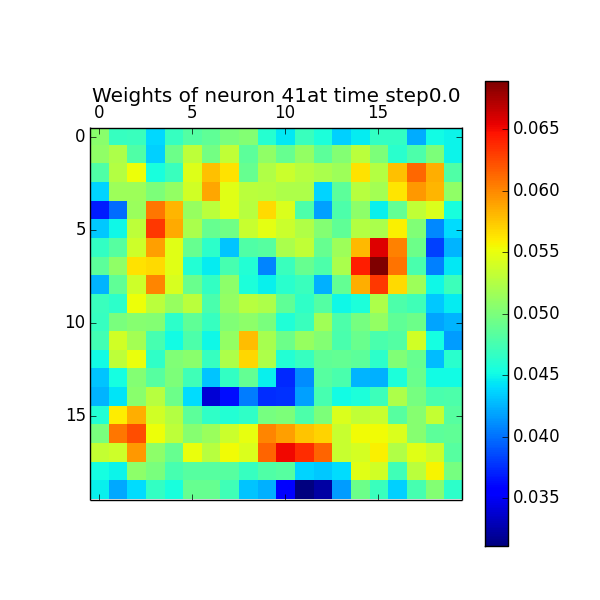
\includegraphics[width=6cm,height=6cm]{neurons/neuron_w_41_t_0.png}\\[10pt]
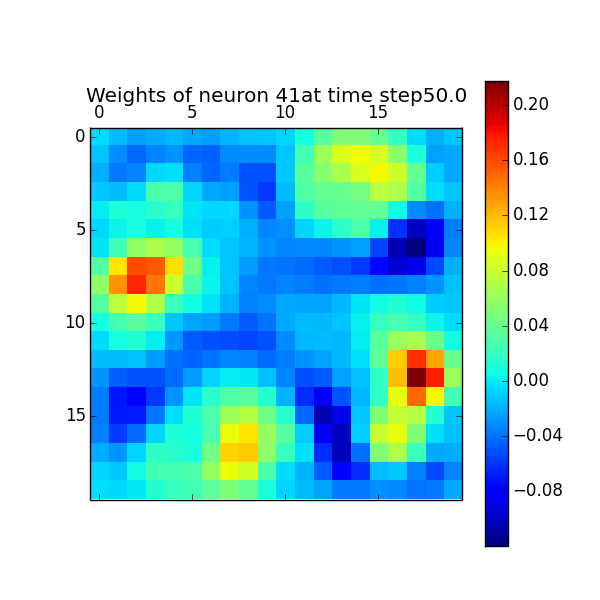
\includegraphics[width=6cm,height=6cm]{neurons/neuron_w_41_t_50.png} \\[10pt]
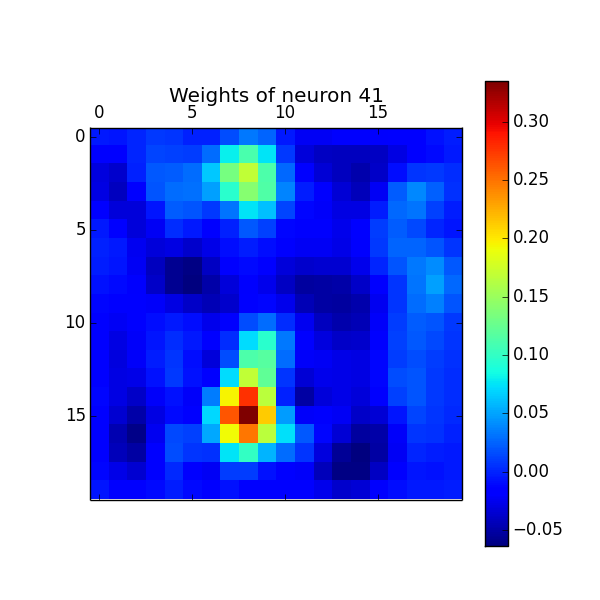
\includegraphics[width=6cm,height=6cm]{neurons/neuron_w_41.png}
        \caption{weight development}
        \label{LabelA}
\end{minipage}
\begin{minipage}[hbt]{0,49\textwidth}
        \centering
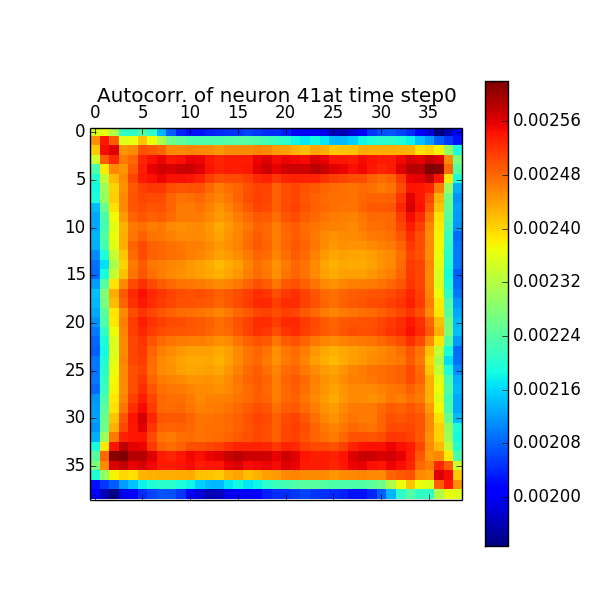
\includegraphics[width=6cm,height=6cm]{neurons/neuron_a_41_t_0.png}\\[10pt]
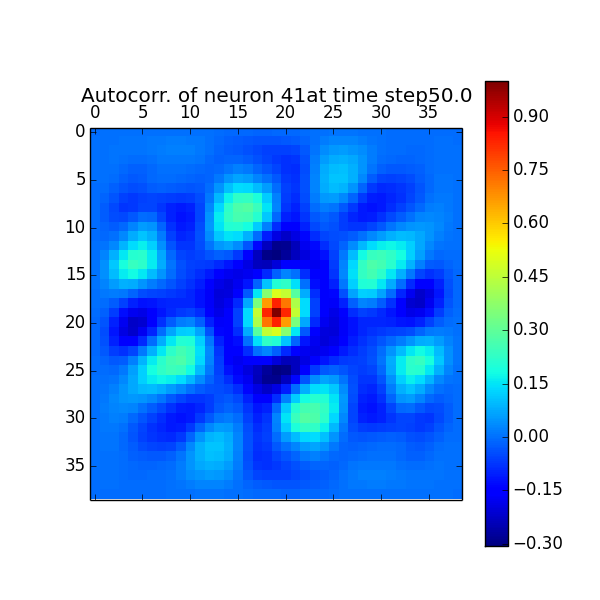
\includegraphics[width=6cm,height=6cm]{neurons/neuron_a_41_t_50.png}\\[10pt]
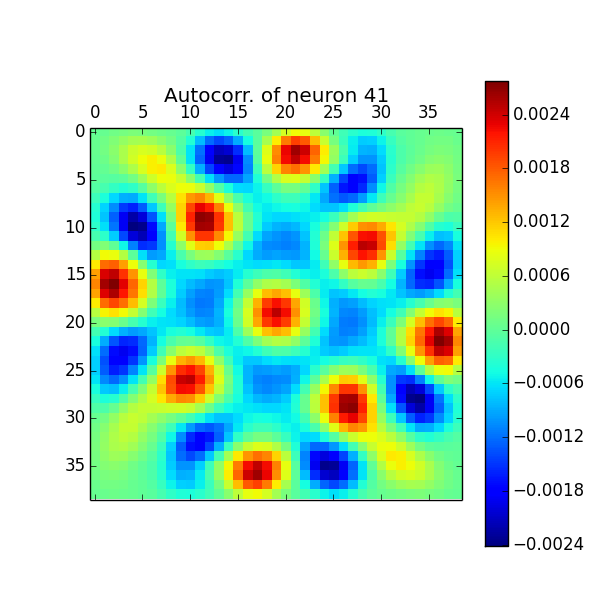
\includegraphics[width=6cm,height=6cm]{neurons/neuron_a_41.png}
        \caption{autocorrellation development}
        \label{LabelB}
\end{minipage}
\centering
\caption{The weights and the autocorrelogram of a neuron at the beginning, middle and the end of the simulation}
\label{time-evol}
\end{figure}

When all grid cells are inspected, it is seen that most grid cells have similar spatial frequencies, however, their orientations and off-sets are different. Figure \ref{diff} illustrates this difference. 

\begin{figure}
\hfill
\subfigure{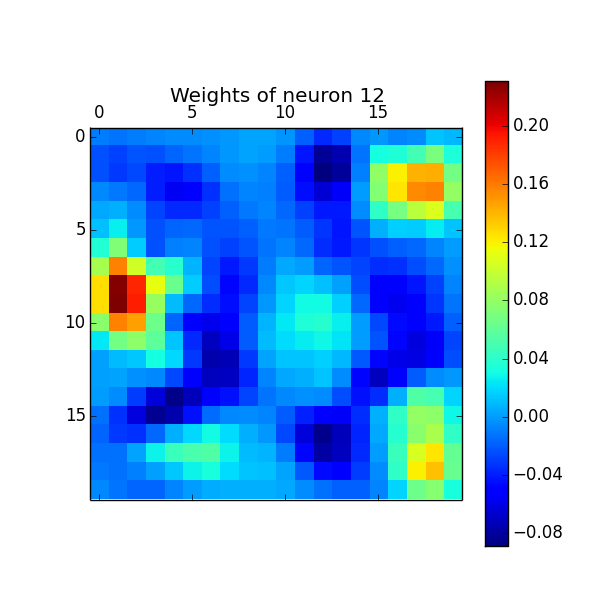
\includegraphics[width=6cm]{neurons/neuron_w_12.png}}
\hfill
\subfigure{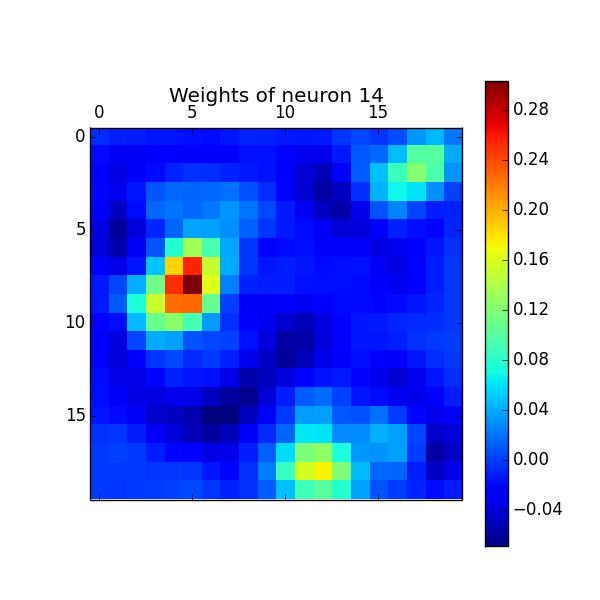
\includegraphics[width=6cm]{neurons/neuron_w_14.png}}
\hfill
\caption{Different grid cells have different orientations and off-sets but similar spatial frequencies.}
\label{diff}
\end{figure}

\section{References}

\end{document}

	